\chapter{Motivation}
\label{chapter2}
\thispagestyle{empty}

\section{Problem statement}
\paragraph{}
In order to avoid Anti-Virus (AV) detection and harden the process of reverse engineering usually malware hide their code employing different techniques. This process, called \textit{packing}, makes the static analysis of a binary almost completely useless.\\
A \textit{packer} is the tool that implements the previously described functions: it receives in input a PE file that represent a Windows program, transforms and obfuscates its code/resources and then appends new codes, called \textit{stub}, that will \textit{unpack} the original one runtime once the program is executed.\\\\

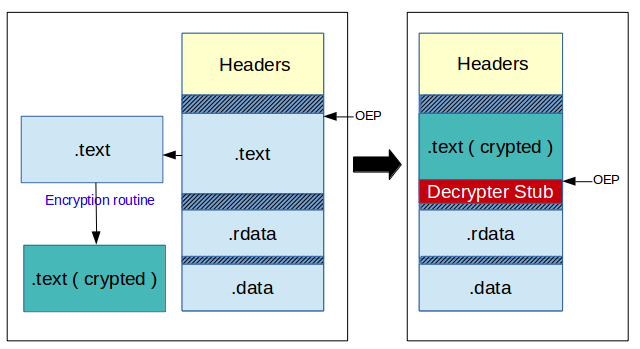
\includegraphics[width=1.1\textwidth]{pictures/packer_general.png} \\\\

The complexity of \textit{packers} can be very different: from those which write and execute directly the original code, to others that employ multiple unpacking routines and obfuscation techniques such as runtime repacking of previously unpacked code.\\
This process has different consequences both in the AV detection and manual analysis of malicious binary:
\begin{itemize}
\item Usually AV employ different static analysis techniques in order to understand if a file is malicious or not, but packing a binary destroys any possibility to understand what the program will do on the system without executing it, and so void any effort from the point of view of a static analysis.
\item The process of reverse engineering a packed malware can be very time consuming and since lots of malware is pushed every day on the internet there is the necessity of fast analysis and fast updating of AV software.
\end{itemize}
\paragraph{}
These problems inspired different works in building an automatic generic unpacker aimed to extract the original code from the packed one. Some of them are more oriented in detection of malicious packed program helping an AV software on end users PCs, others are instead proposed as tools for speed up the work of professional malware analysts.
\paragraph{}
A comprehensive study and a taxonomy of the levels of complexity of nowadays packers have been presented by Ugarte-Pedrero et al\cite{sokpacker}. 
In order to clarify better what a packer is and how it operates we will discuss in the next capther the main points of the previously mentioned research.

\subsection{Packer taxonomy}
\paragraph{}
As previously explained a packer can implements different obfuscation techniques in order to harden the analysis of a program. In this capther we are going to analyze the proposed taxonomy in order to better understand the goals of our work and its limitation against the current packing methods.

Before starting to present the techniques we need to define some terms that are essential in order to understand how a packer works: 
\begin{itemize}
\item \textit{Layer}: a layer is a set of contiguous memory addresses that are executed after being written.A layer can unpack another unpacking-layer or layer that contains the original program code.
\item \textit{Transition}: a transition is a control transfer from a layer to another layer, it can be a \textit{forward transition} if the execution is going from a previously unpacked layer to a newer layer, or a \textit{backward transition} if the execution is going from a newer layer to an older one. From this definition we can derive the concept of \textit{linear unpacking} in which all the transition are \textit{forward transition}, and {cyclic unpacking} in which there are some \textit{forward transition} and some \textit{backward transition}. 
\item \textit{Tailed/Interleaved}: We say that a packer is tailed if there is soon or later a transition from the unpacking layers to the original program code and then the execution never returns to the unpacking layers, contrary we say that the unpacking is \textit{interleaved} if the execution bounce between the unpacking layers and the original program code. 
\item \textit{Frame}: a frame is a portion of original program code, if a packer is \textit{mono frame} that means that the unpacking routine will reveal all the original code before jumping and executing it; contrary a \textit{multi frame} packer unpack only a slice of the original program code, execute it and then unpack another slice of original program code and so on. A \textit{multi frame} behavior can be \textit{incremental} if the slices of original program are revelead in order following the original program execution and never re-encrypted again, contrary a \textit{shifted frames} policy reveal only one slices at times and re-encrypt the slice once executed.
\end{itemize}

As proposed by Ugarte-Pedrero et al\cite{sokpacker} we are going to identify the complexity of a packer by using a scale from 1 to 6.

\subsubsection{Type 1}

The simplest form of packer is the one that runtime unpack the original binary using 
only one layer and then jumps to it with a tail jump. \\

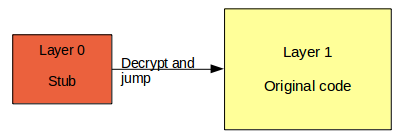
\includegraphics[width=0.7\textwidth]{pictures/packer_type_1.png} 

This scheme is typical of packers like UPX,FSG,EXEpacker.

\subsubsection{Type 2}

The packer in this category are defined as \textit{multi-layer} and \textit{linear}. This means that they employ different layer and the transition between them is always from the older to the newer. Also this kind of packers are defined as \textit{tailed} since the last jump redirect the execution at the original program code.

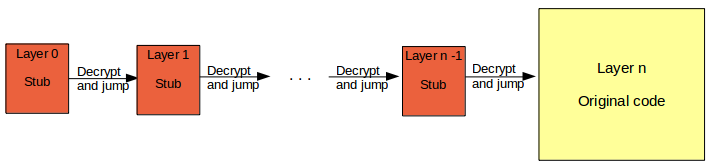
\includegraphics[width=1.2\textwidth]{pictures/packer_type_2.png}

\subsubsection{Type 3}

Type 3 packers are defined as \textit{multi-layer}, \textit{cyclic} and \textbf{tailed}. This means that they employ different layers and the transitions are both \textit{forward transition} and \textit{backward transition}.  

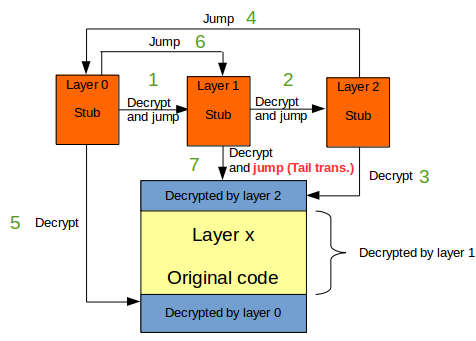
\includegraphics[width=1\textwidth]{pictures/packer_type_3.png} 

\subsubsection{Type 4}

These packers are \textit{multi-layer}, \textit{cyclic} and \textit{interleaved}. This means that they use different layers with both \textit{forward and backward transitions}, and during the execution of the original program the control is redirected in some way to the packer code.

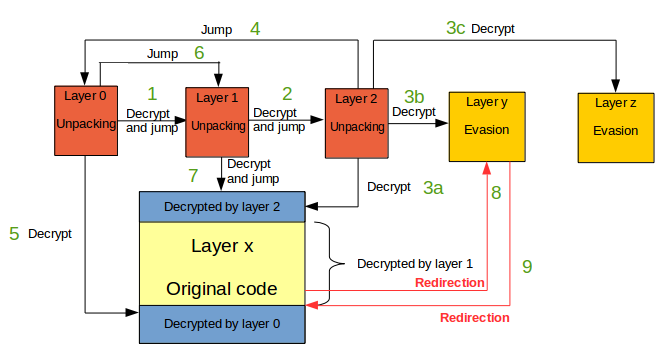
\includegraphics[width=1.07\textwidth]{pictures/packer_type_4.png} 

\subsubsection{Type 5}

Packers of this type are \textit{multi-layer}, \textit{cyclic},\textit{interleaved} and \textit{multi frame} with an \textit{incremental frames} behavior. This means that they use different layers with both \textit{forward and backward transitions}, during the execution of the original program the control is redirected in some way to the packer code and the original program code is revelead slice by slice when need to execute; also for this packers there is a moment in which all the original program code is in memory, so dumping at the original entry point doesn't permit to dump all the original program code since it is still encrypted in memory, but a theoretical dump nearly the end of execution can dump the entire program's code.

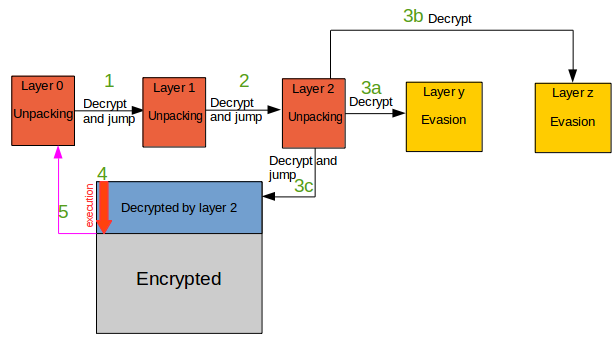
\includegraphics[width=1\textwidth]{pictures/packer_type_5-1.png}

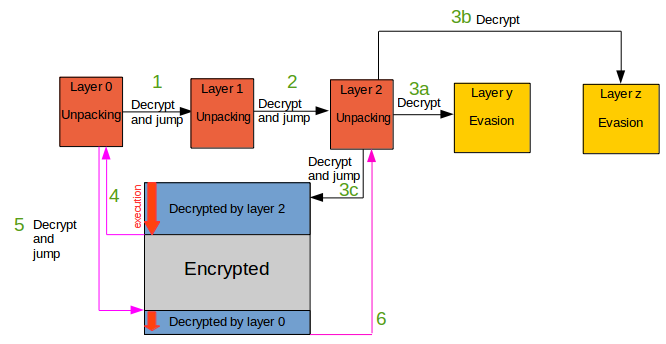
\includegraphics[width=1.1\textwidth]{pictures/packer_type_5-2.png}

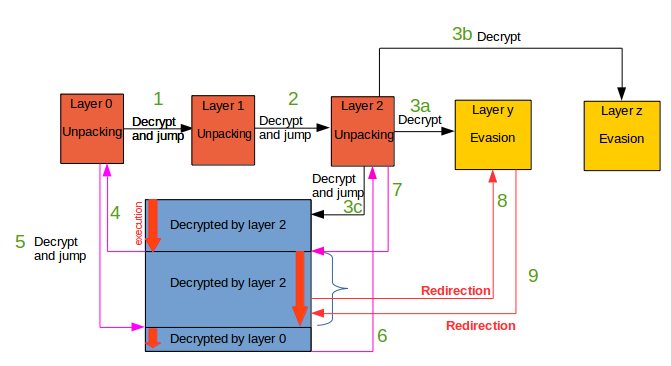
\includegraphics[width=1.1\textwidth]{pictures/packer_type_5-3.png}


\subsubsection{Type 6}

Packers of this type are \textit{multi-layer}, \textit{cyclic},\textit{interleaved} and \textit{multi frame} with a \textit{shifted frames} behavior. This means that they use different layers with both \textit{forward and backward transitions}, during the execution of the original program the control is redirected in some way to the packer code and the original program code is revelead slice by slice and re-encrypted once executed; packers with such complexity never let all the program code to live in memory, so a dump that encompass the entire original program's code doesn't exists.

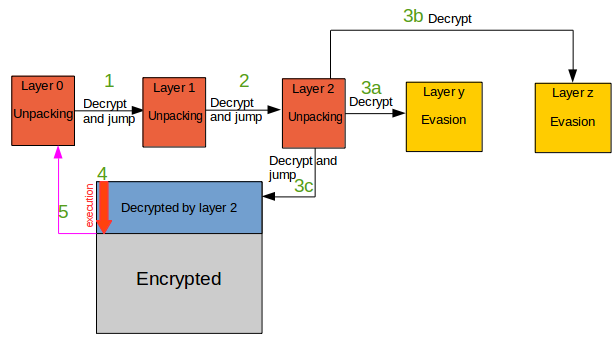
\includegraphics[width=1\textwidth]{pictures/packer_type_5-1.png}

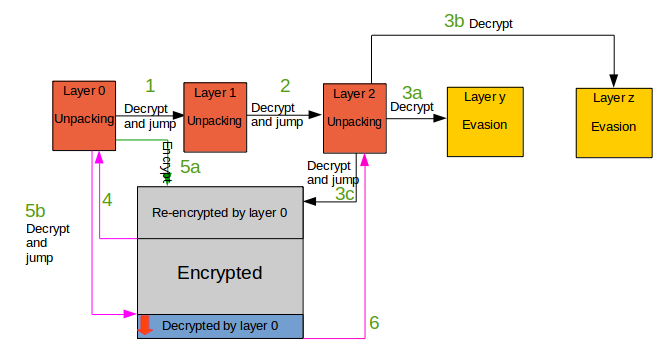
\includegraphics[width=1.05\textwidth]{pictures/packer_type_6-1.png}

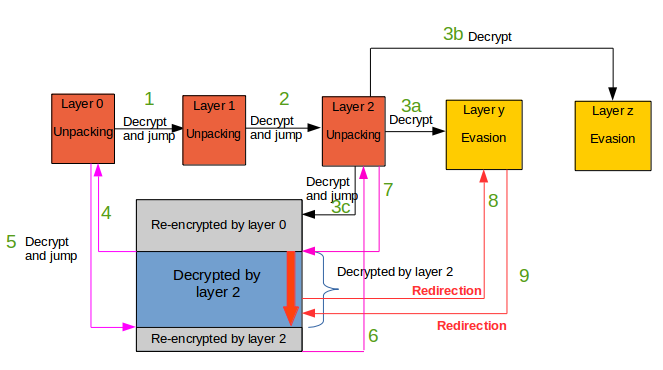
\includegraphics[width=1.05\textwidth]{pictures/packer_type_6-2.png}

\section{State of the art}
\paragraph{}
Lots of different tools using different approaches and techniques have been proposed. 
The approaches for automatic unpacking can be very different:
\begin{itemize}
\item \textit{Static unpacking}: this can sound counterintuitive, but some works proposed to identify unpacking routines inside the binary and reconstruct an ad hoc unpacker for the binary starting from these routines. This approach has got numerous limitation but can lead to interesting result in some case as demonstrated by Caballero et al.
\item \textit{Hybrid unpacking}: this mixes some static heuristics with dynamic analysis.
\item \textit{Dynamic unpacking}: these techniques follow the idea to let the unpacker do its work and then try to extract runtime the unpacked code. 
\end{itemize}
\paragraph{}
Depending on the purpose of the tool there are different requirements that a generic unpacker must respect. If the aim is to help the AV on end users' PCs:
\begin{itemize}
\item Safety: try to recognize the malicious behaviour as fast as possible and block the execution. 
\item Performance: it should not slow down too much the execution of AV scans.
\end{itemize}
Note that in these cases, the scope is not to reconstruct a binary from a packed one, but rather to stop malicious behaviours when they manifest. \\
In this area have been done works such as OmniUnpack and JustIn.
\paragraph{}
On the other side if the aim is to help the analysis in a laboratory:
\begin{itemize}
\item Fidelity: the unpacked binary extracted by the tool should be equal to the one that would be unpacked normally. 
\item Generality: the unpacker can not be focused only against one packer but should unpack different of them with one generic algorithm.
\end{itemize}
In this case we do not care so much about safety because usually analysis is performed inside a controlled environment and the analysts want to observe the complete execution of malware. Also the performances are not a critical feature here because we are not constrained by user experience needs.\\
In this category have been developed tools like PolyUnpack, Ether, Eureka, Renovo, Lynx.
These tools merely collect dumps of the binary while unpacking and they don't reconstruct a fully runnable binary given a packed one.


\section{Goals and challenges}
\paragraph{}
Since our work is born as a component of a bigger malware analysis platform (Jackdaw), our tool is oriented to help malware analyst during the reversing process of a packed binary. 
Our approach aims not only to unpack the malware, but also to reconstruct a fully working unpacked binary. To do so, we not only have to identify the original entry point (OEP) and dump the code at that moment, but we have to find the IAT inside the process and reconstruct a correct import directory in the final PE file.\\
The first thing we have to deal with are the unpacking routines of the packers: every time the execution of the malware comes from a previously written memory area, then it could be a sign that the unpacking stage has finished or that a new unpacking layer has started.\\
We have also to deal with techniques of IAT obfuscation: some malwares can do this in order to make difficult to statically analyse them to understand what they are doing.

